\documentclass[11pt,a4paper]{article}
\usepackage[hyperref]{acl2018}
\usepackage{times}
\usepackage{latexsym}
\aclfinalcopy % Uncomment this line for the final submission
%\def\aclpaperid{***} %  Enter the acl Paper ID here

%\setlength\titlebox{5cm}
% You can expand the titlebox if you need extra space
% to show all the authors. Please do not make the titlebox
% smaller than 5cm (the original size); we will check this
% in the camera-ready version and ask you to change it back.

\usepackage{graphicx} % for imports
\usepackage{subcaption} % for figures
\usepackage{cleveref}
\graphicspath{{img/}}
\usepackage{pgfplots} % plotting pgf format directly
% citations

\title{Planning Paper}

\author{Luis Glaser\\
  registration number 800140 \\
  Potsdam University \\
  {\tt Luis.Glaser@uni-potsdam.de} \\
  \\
  Advanced Natural Language Processing (WS 2018/2019) \\
  Dr. Tatjana Scheffler \\
  \\}

\date{11. January 2019}
\usepackage{url}

\begin{document}
\maketitle

\thispagestyle{plain}

\section*{Introduction \& Motivation}

Together with Atreya Shankar and Juliane Hanel I will work on music lyrics. The original motivation was our shared interest in music and the different social and political dimension that can be expressed through it. Although music also consists of the audio signal, lyrics do play an important role when analysing. E.g. \citet{fell_lyrics-based_2014} noted, that considering lyrics in recommendation engines does increase their quality.

This suggests, that we should be able to find meaningful patterns when using the lyrical data only. After generating an initial dataset, we had different questions in mind. These included but were not limited to: Is there a significant difference between rap and pop lyrics? How do different genres differ in their emotionality? How have music lyrics in general evolved over time? 

As it should be clear by know, we will take a broad approach and try to answer an array of questions all concerned with music lyrics.

This planning paper serves the purpose of structuring those initial questions, in order to keep our research focused. It also will give an overview of what we currently have planned and which areas we still need to work on. 

\section*{Method}\label{sec:method}
\begin{figure}[h]
	\centering
	\resizebox{\linewidth}{!}{
		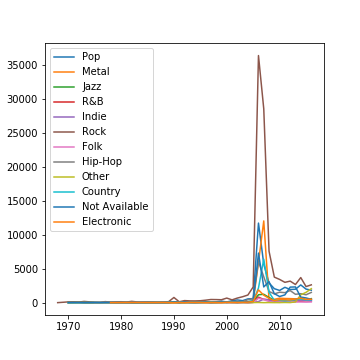
\includegraphics{img/kaggleplot_bias}
	}
	\caption{Distribution of genre over time in \texttt{kaggle} data}
       \label{fig:kaggle}
\end{figure}

When first experimenting with our ideas, we went with the first available dataset we found on Google's Dataset Search\footnote{\url{https://toolbox.google.com/datasetsearch}} \citep{kuznetsov_55000+_2017}. However, we came across initial flaws, as the dataset was very biased towards a certain year. This can easily be seen in the histogram depicted in \cref{fig:kaggle}. Thus, we will not use this in the end. We currently have two approaches we considering taking from here.

The first one will be to crawl data by ourselves by interfacing with the genius API.\footnote{\url{https://docs.genius.com}} The work on this crawler is still in progress and we can't yet tell if this dataset will have less of a bias. The second technique will be to search for further datasets and integrate them into one dataset. This would have multiple disadvantages. First, it's likely that we won't be able to completely get rid of the bias and second will introduce new challenges like merging the data and unifying their formats. This wouldn't provide anything interesting for us to learn. Thus we hope our crawler will return a satisfactory dataset.

\section*{Tooling}
\begin{figure}[h!]
	\centering
	\scriptsize
	\begin{tabular}{llllll}
ID & Artist & Title & Year & Genre & Lyrics \\
1 & Rihanna & Diamonds & 2012 & Pop & Shine bright $\ldots$ \\
2 & Toto & Africa & 1982 & Pop & I hear the drums $\ldots$ \\
	\end{tabular}
	\caption{Example entries in \texttt{SQLite} database}
	\label{fig:table}
\end{figure}
For data house keeping we will use a \texttt{SQLite}\footnote{\url{https://www.sqlite.org}} database which will be shared over \texttt{GitHub} and interfaced via \texttt{python}. Furthermore as mentioned already in our group contract, we will use this \texttt{GitHub} repository for collaboration in general. 
One of my responsibilities will be to detect and annotate political sentiment expressed in lyrics. Right now I intend to use a \texttt{Word2Vec} \citep{mikolov_efficient_2013} to represent lyrics and extrapolating their political expression from their. However, how to validate our results is still unclear and will need more work in the upcoming weeks.

\thispagestyle{plain}
\section*{Personal Contribution}

I will contribute to this project on multiple different ends. 

I will be responsible of taking care of our database system. In both my undergraduate degrees I had had to work with rather large datasets that kept changing during work. Thus, I am familiar with a few pitfalls concerning data handling. My work should ensure that all of us can work undisrupted and not have to bother a lot with the usual data juggling. 

As noted before, we do not have a proper data set yet. Thus, another task for me will be to build the crawler with which we will collect the lyrics. I have never programmed a crawler before, but worked on post processing modules within a larger web crawler. Therefore I bring a fair amount of experience with me while having my colleagues as a backup in case we need help.

Furthermore I will take care of annotating political expressions to the lyrics (if) they are expressed. I wanted to do this within my undergrad thesis in political science already. Unfortunately, I didn't get around to it since it was beyond the scope for doing it for German data. This will be a interesting challenge for me, since it gets harder as more dimensions need to be taking into account \cite{cohen_classifying_2013}. 

In general, I already worked with quite a few of the annotations that we will create during our analysis. Thus, I should be able to contribute my experience in that area and provide help to my fellow teammates. 

After our annotation phase, I will join Atreya and Juliane with the change analysis. I will aim at bringing my traditional engineering background to the table, trying to solidify our results with sceptical thinking. However, I feel Atreya and Juliane have way more experience then me in this field, which I hope to profit from.

\section*{Learning Goals}

This brings us to the personal learning goals.
Our project will use quite a few techniques that were discussed in class. These entail word frequency analysis and part of speech tag analysis. Beyond these, sentiment analysis and vector representations are discussed in our textbook \cite{jurafsky2014speech}. 

Therefore, our final project will give us the ability to deepen our understanding of these topics. Also using them on our own dataset and with our own research questions should strengthen our intuition of these methods.
We also will be able to try out new methods which will help us when deciding on classes within the rest of our masters programme. This is especially true for the rather exploratory approach that we intend to take. Each hypothesis can be tested in a fairly short amount of time. Testing multiple highly different hypothesis will give us all the opportunity to try and get first or second experience with the techniques that we will employ. This should create an ideal learning basis for the upcoming weeks and the finale of this course.


\bibliography{bibtex}
\bibliographystyle{acl_natbib}


\end{document}

